% Model 3 structure (paper Fig. "Structure of Model 3").
% Matches m1_structure.tex and m2_structure.tex 4-column architecture & paper_palette.
% Build: cd Paper/Figure && pdflatex m3_structure.tex
\documentclass[tikz,border=3pt]{standalone}
\usepackage{newtxtext,newtxmath}
\usepackage{amsmath,bm}
\usetikzlibrary{arrows.meta,calc,backgrounds}
% Shared colours for the TikZ schematics; same roles and hex values as
% Code/figures_matlab/paper_style.m (mycolor.space, base #1E5F74).
%   water (P, I, M, W-bar)  teal   | vegetation (V, r, d)  green
%   wind and sand (E, S)    brown  | highlight             orange
%   limits and caps         red dashed
\definecolor{pWater}{HTML}{1E5F74}
\definecolor{pWaterMid}{HTML}{659FB6}
\definecolor{pWaterLight}{HTML}{DCEBF1}
\definecolor{pTeal}{HTML}{00828C}
\definecolor{pVeg}{HTML}{2B633C}
\definecolor{pVegMid}{HTML}{4AC087}
\definecolor{pVegLight}{HTML}{E3F3E8}
\definecolor{pSand}{HTML}{8F7159}
\definecolor{pSandLight}{HTML}{FFEACE}
\definecolor{pAccent}{HTML}{F49431}
\definecolor{pPV}{HTML}{D47216}
\definecolor{pPVLight}{HTML}{FDF1E3}
\definecolor{pPlum}{HTML}{7A437F}
\definecolor{pPlumLight}{HTML}{F2EBF3}
\definecolor{pLimit}{HTML}{D03B3B}
\definecolor{pInk}{HTML}{1F2B33}
\definecolor{pAxis}{HTML}{344A53}
\definecolor{pGrey}{HTML}{97AFB9}
\definecolor{pGreyDark}{HTML}{647B84}
\definecolor{pGrid}{HTML}{E6EBED}

\tikzset{
  box/.style={rectangle, rounded corners=2.5pt, line width=0.8pt, align=center,
    font=\small, inner xsep=4pt, inner ysep=3.2pt, minimum height=0.84cm,
    execute at begin node={\hyphenpenalty10000 }},
  data/.style={box, draw=#1, fill=white, text=pInk},
  step/.style={box, draw=#1, fill=#1!10, text=pInk},
  core/.style={box, draw=#1, fill=#1, text=white, font=\small\bfseries, minimum height=0.96cm},
  result/.style={box, draw=#1, fill=#1, text=white},
  capbox/.style={box, draw=pLimit, dash pattern=on 3.5pt off 2pt, fill=pLimit!6, text=pInk},
  flow/.style={-{Stealth[length=5pt,width=4pt]}, line width=0.8pt, draw=#1},
  flow/.default=pAxis,
  colhead/.style={font=\footnotesize\bfseries, text=pGreyDark, anchor=south},
}
\begin{document}
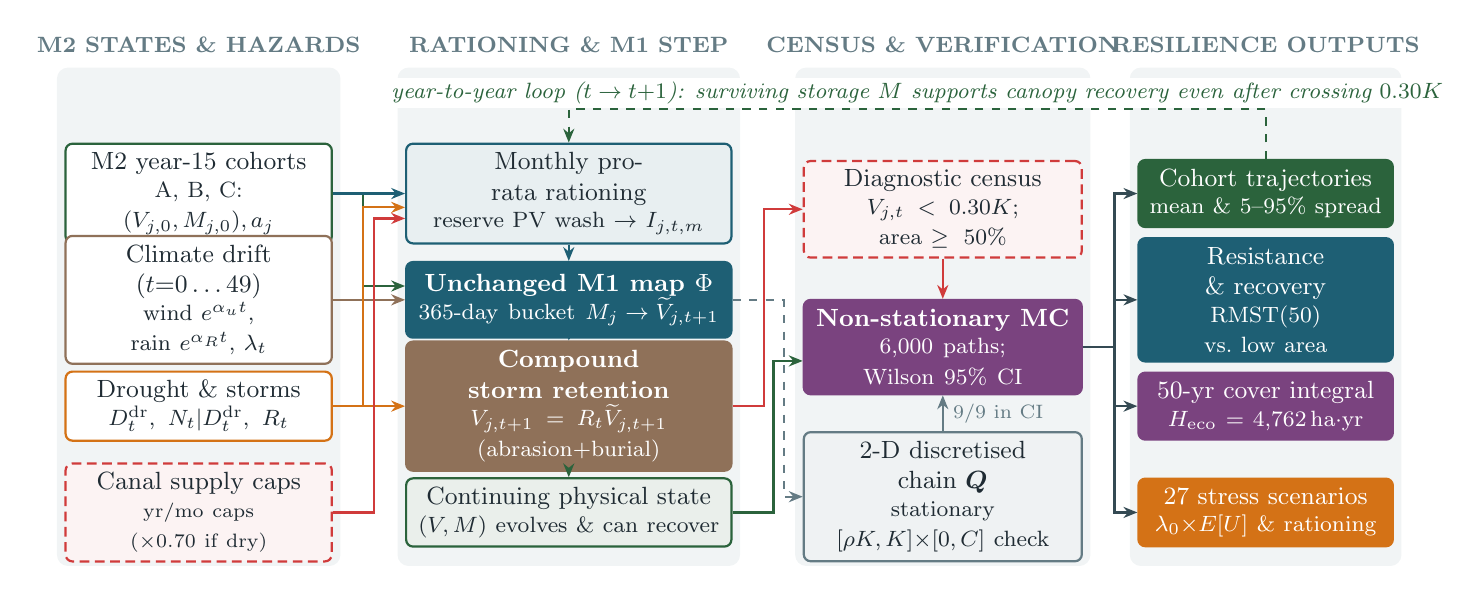
\begin{tikzpicture}
% ---- column headings
\node[colhead] at (1.90,0.72)  {M2 STATES \& HAZARDS};
\node[colhead] at (6.60,0.72)  {RATIONING \& M1 STEP};
\node[colhead] at (11.35,0.72) {CENSUS \& VERIFICATION};
\node[colhead] at (15.45,0.72) {RESILIENCE OUTPUTS};

% ---- column 1: inherited states & nonstationary hazards
\node[data=pVeg,   text width=3.1cm] (init)  at (1.90,-0.95) {M2 year-15 cohorts\\[-1pt]{\footnotesize A, B, C: $(V_{j,0},M_{j,0}),a_j$}};
\node[data=pSand,  text width=3.1cm] (trend) at (1.90,-2.30) {Climate drift ($t{=}0\dots49$)\\[-1pt]{\footnotesize wind $e^{\alpha_u t}$, rain $e^{\alpha_R t}$, $\lambda_t$}};
\node[data=pPV,    text width=3.1cm] (shock) at (1.90,-3.65) {Drought \& storms\\[-1pt]{\footnotesize $D_t^{\mathrm{dr}},\ N_t{\mid}D_t^{\mathrm{dr}},\ R_t$}};
\node[capbox,      text width=3.1cm] (caps)  at (1.90,-5.00) {Canal supply caps\\[-1pt]{\scriptsize yr/mo caps ($\times0.70$ if dry)}};

% ---- column 2: within-year rationing & physical update
\node[step=pWater, text width=3.85cm] (rat)  at (6.60,-0.95) {Monthly pro-rata rationing\\[-1pt]{\footnotesize reserve PV wash $\to I_{j,t,m}$}};
\node[core=pWater, text width=3.85cm] (phi)  at (6.60,-2.30) {Unchanged M1 map $\Phi$\\[-1pt]{\footnotesize\normalfont 365-day bucket $M_j \to \widetilde V_{j,t+1}$}};
\node[core=pSand,  text width=3.85cm] (hit)  at (6.60,-3.65) {Compound storm retention\\[-1pt]{\footnotesize\normalfont $V_{j,t+1}=R_t\widetilde V_{j,t+1}$ (abrasion+burial)}};
\node[step=pVeg,   text width=3.85cm] (rec)  at (6.60,-5.00) {Continuing physical state\\[-1pt]{\footnotesize $(V,M)$ evolves \& can recover}};

% ---- column 3: annual census, MC & 2-D Markov cross-check
\node[capbox,        text width=3.25cm] (cen) at (11.35,-1.15) {Diagnostic census\\[-1pt]{\footnotesize $V_{j,t}<0.30K$; area $\ge50\%$}};
\node[core=pPlum,    text width=3.25cm, minimum height=1.08cm] (mc) at (11.35,-2.90) {Non-stationary MC\\[-1pt]{\footnotesize\normalfont 6,000 paths; Wilson 95\% CI}};
\node[step=pGreyDark,text width=3.25cm] (mk)  at (11.35,-4.80) {2-D discretised chain $\bm Q$\\[-1pt]{\footnotesize stationary $[\rho K,K]{\times}[0,C]$ check}};

% ---- column 4: outputs
\node[result=pVeg,   text width=2.95cm] (p1) at (15.45,-0.95) {Cohort trajectories\\[-1pt]{\footnotesize mean \& 5--95\% spread}};
\node[result=pWater, text width=2.95cm] (p2) at (15.45,-2.30) {Resistance \& recovery\\[-1pt]{\footnotesize RMST(50) vs.\ low area}};
\node[result=pPlum,  text width=2.95cm] (p3) at (15.45,-3.65) {50-yr cover integral\\[-1pt]{\footnotesize $H_{\mathrm{eco}}=4{,}762$\,ha$\cdot$yr}};
\node[result=pPV,    text width=2.95cm] (p4) at (15.45,-5.00) {27 stress scenarios\\[-1pt]{\footnotesize $\lambda_0{\times}\mathbb E[U]$ \& rationing}};

% ---- flows
\draw[flow=pVeg]   (init.east)  -- ++(0.38,0) |- ([yshift=5pt]phi.west);
\draw[flow=pWater] (init.east)  -- (rat.west);
\draw[flow=pSand]  (trend.east) -- (phi.west);
\draw[flow=pPV]    (shock.east) -- (hit.west);
\draw[flow=pPV]    (shock.east) -- ++(0.38,0) |- ([yshift=-5pt]rat.west);
\draw[flow=pLimit] (caps.east)  -- ++(0.52,0) |- ([yshift=-9pt]rat.west);

\draw[flow=pWater] (rat.south)  -- (phi.north);
\draw[flow=pWater] (phi.south)  -- (hit.north);
\draw[flow=pVeg]   (hit.south)  -- (rec.north);

\draw[flow=pLimit] (hit.east)   -- ++(0.40,0) |- (cen.west);
\draw[flow=pVeg]   (rec.east)   -- ++(0.52,0) |- ([yshift=-5pt]mc.west);
\draw[flow=pLimit] (cen.south)  -- (mc.north);
\draw[flow=pGreyDark, dashed] (phi.east) -- ++(0.65,0) |- (mk.west);
\draw[flow=pGreyDark] (mk.north) -- node[right, font=\scriptsize, text=pGreyDark] {9/9 in CI} (mc.south);

\draw[flow] (mc.east) -- ++(0.40,0) |- (p1.west);
\draw[flow] (mc.east) -- ++(0.40,0) |- (p2.west);
\draw[flow] (mc.east) -- ++(0.40,0) |- (p3.west);
\draw[flow] (mc.east) -- ++(0.40,0) |- (p4.west);

% ---- top feedback arc: physical recovery loop across years t -> t+1
\draw[flow=pVeg, dashed] (p1.north) -- (15.45, 0.12)
  -- node[above, font=\footnotesize\itshape, text=pVeg, fill=white, inner sep=1.5pt]
     {year-to-year loop ($t\to t{+}1$): surviving storage $M$ supports canopy recovery even after crossing $0.30K$}
  (6.60, 0.12) -- (rat.north);

% ---- light column bands
\begin{scope}[on background layer]
  \foreach \x/\w in {1.90/3.6, 6.60/4.35, 11.35/3.75, 15.45/3.45}
    \fill[pGrid!55, rounded corners=4pt] (\x-\w/2,0.65) rectangle (\x+\w/2,-5.68);
\end{scope}
\end{tikzpicture}
\end{document}
